\section{Implementation}

\subsection{Arena setup}

In the model implemented, an ANN with fixed architecture was used, see Fig. \ref{fig:NN}. A genetic algorithm was used to optimise the weights of the ANN, evolving the desired rat behaviour. 

The simulated elevated plus maze was discretised into 15 positions as shown in Fig. \ref{fig:arena-disc}. This was inspired by a similar, proven solution detailed within \citeauthor{Costa201444} and \citeauthor{Costa2016102}. \cite{Costa201444} \cite{Costa2016102} GPS ranges from the E-puck were assigned EPM positions in order to provide the robot's position to the supervisor.


\begin{figure}[H]
	\centering
	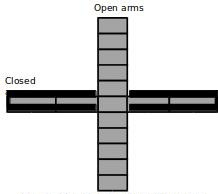
\includegraphics[width=0.7\linewidth]{arena-disc}
	\caption{Arena boundaries}
	\label{fig:arena-disc}
\end{figure}

\subsection{Robot controller}

The e-puck is controlled by a multilayer perceptron (MLP), shown in Fig. \ref{fig:NN} with arrows representing weighted links. 

The network's inputs are data from the circumferential IR proximity sensors. The outputs of the network specify wheel speed values. 

In terms of activation functions, every neuron uses a hyperbolic tangent function. This suited this application as this function’s output is between -1 and 1, which is ideal because wheel speeds can be negative. The output values are scaled by 1000, to match the possible range of values in wheel speeds.

Each layer of synaptic weights is represented by an N-by-N matrix, where each row is a neuron's connection's weights to the next layer. \cite{Seiffert2001} These individual sets of weights are encoded into another data structure, which contain the weights of each layer. 

\subsection{Evolution}

The network's weights are optimised by a genetic algorithm. 

Each individual of the population is evaluated by the GA. As stated, each individual is a separate robot controller (ANN), with different parameters (weights).

The population is initialised via a function that fills a matrix with uniformly distributed random numbers in the range of -1 to 1, which are the initial weights. The size of the initial population is dictated by the variable \emph{popsize}. 

The fitness of each individual is evaluated with a fitness function. At each time step, this takes in as input the position of the robot and the proximity sensor values. The fitness value assigned to a controller under evaluation is increased or decreased depending on whether it exhibited desirable or undesirable behaviour. The algorithm awards ``rat-like'' behaviour such as predominantly staying within the confines of the enclosure (anxious exploratory behaviour) and close to walls, and punishes falling off the arena, exploring the outer boundaries of the arm and wall collisions.

Each individual is evaluated after navigating through the virtual EPM for 30 seconds.

Successive generations are created through selection and reproduction of the previous generation.

Based on the fitness of these individuals, the best individuals are selected by elitism and the remaining individuals are selected through tournament selection. 

In elitism, a proportion of the best individuals are copied directly to the new generation, and the percentage for which this is done is dictated by the variable \textit{elitism}. 

In tournament selection, a number of individuals are chosen randomly, according to the variable \textit{tournamentSize}. These individuals are sorted by their fitness and the best two are chosen as parents. 

A new individual is reproduced using uniform crossover. In uniform crossover, there is a 50\% probability that the current gene is selected from one parent and not the other. 

Gaussian mutation is also applied with a probability dictated by the variable \textit{muteRate} (i.e. the number of individuals in a generation to be mutated) and with severity dictated by the variable \textit{severity} (i.e. the number of genes in the individual to be mutated). The variables mentioned above are all user definable.

When the best controller is evolved, the final generation of individuals is sorted by fitness and saved to an .xml file for analysis and reuse.

\subsection{Simulation supervisor}

The supervisor acts as a tool to guide and control the simulation. The user first sets the desired mode of operation (demo or evolution). Then the supervisor sets the time step of the current simulation as well as the duration of time each controller should run for, and resets the robot to its initial position.  

